\subsection{$k$-Nearest Neighbours}
\label{sec:knn}
%\knn{} is a well known method in supervised learning, it is a 
%non-parametric method and a type of instance-based learning, or lazy 
%learning .\\

%The overall \knn{} concept is simple: store the whole training set 
%in 
%the memory space, calculate the distance between the given test 
%point 
%to all training points, and apply the majority voting system to 
%determine which class the test data sample belongs to.
One of the advantages of using \knn{} is that it is 
intuitive and simple. Moreover, \knn{} algorithm has no training 
phase. 
However, \knn{} stores all training data in the memory space, 
therefore, the method will become slower as the training data 
increase, see Figure~\ref{fig:knncomp}.
We used 
a standard binary 0-1 loss to determine the overall 
accuracy and confusion matrix of the model, see Table~\ref{tbl:res}.
Figure~\ref{fig:knnerror} shows the training and test errors with 
respect to the number 
of neighbours $k$ (X-axis). 
%Test error has the smallest value of $0.0563$ when $k=3$.

In addition to the standard \knn{}, we implemented a second version 
of 
\knn{} algorithm that is more 
robust to unstable features. This implementation uses Minkowski 
distance with parameter $p=3$. More details can be found in the 
provided MATLAB code. 

%First, we input the extracted ECG signal's features data into the 
%algorithm, then it stores the training set. Second we input the 
%testing data into the algorithm, and perform distance calculation 
%between every points. This time we use Minkowski distance with a 
%parameter being 3 to increase its robustness to unstable features.

\paragraph{Implementation.}
MATLAB was used to program the \knn{} algorithm. No additional 
libraries or tools required. 

\begin{figure}
	\centering
	\begin{subfigure}{.37\textwidth}
		\centering
		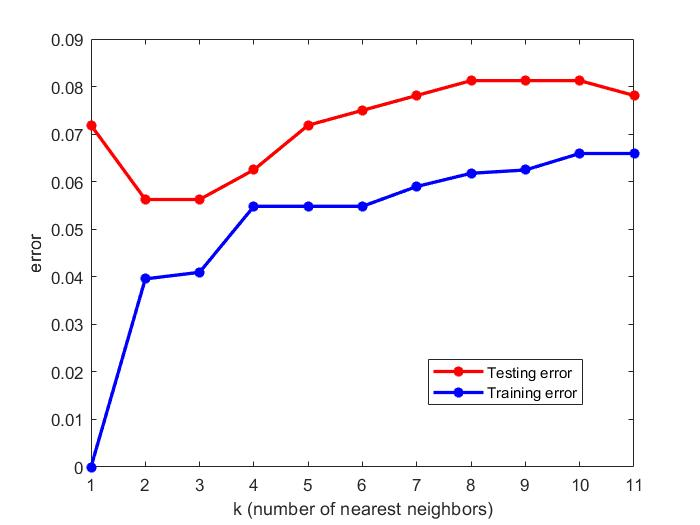
\includegraphics[width=.9\linewidth]{figures/knnerror.jpg}
		\caption{Error Plot}
		\label{fig:knnerror}
	\end{subfigure}%
	\begin{subfigure}{.37\textwidth}
		\centering
		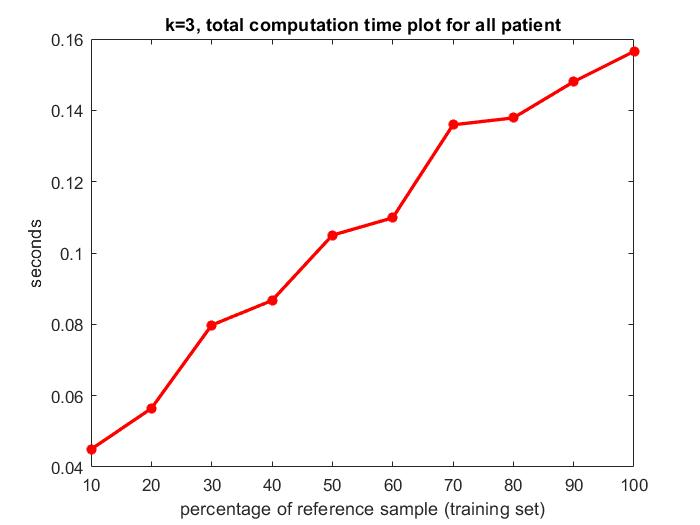
\includegraphics[width=.9\linewidth]{figures/kNNpercentage.jpg}
		\caption{Computation Time}
		\label{fig:knncomp}
	\end{subfigure}
	\caption{\knn{} performance: training/test errors (left) and 
	computation time (right).}
	\label{fig:knn}
\end{figure}

%\begin{figure}[t]
%	\centering
%	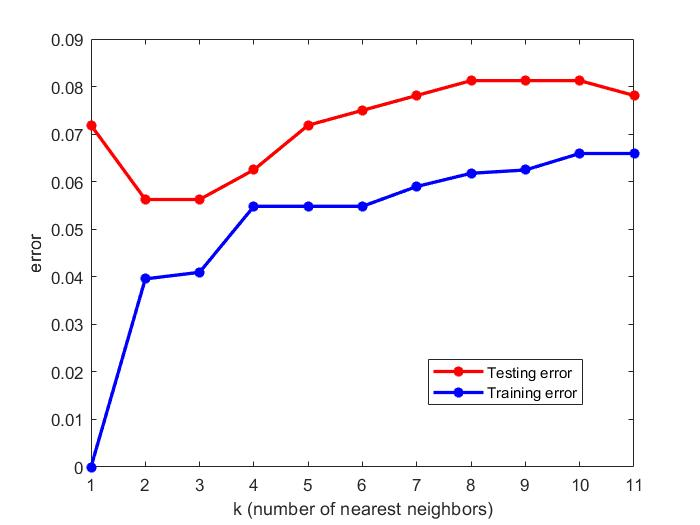
\includegraphics[width=0.6\textwidth]{figures/knnerror.jpg}
%	\caption{Error Plot}
%	\label{fig:knnerror}
%\end{figure}

%\begin{figure}[t]
%	\centering
%	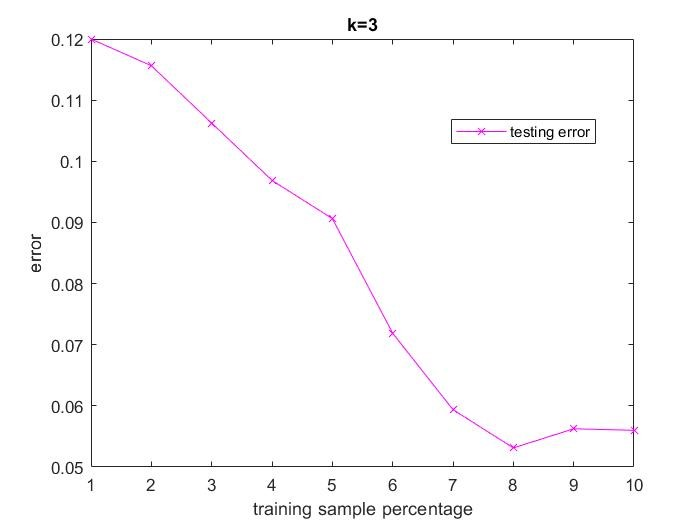
\includegraphics[width=0.6\textwidth]{figures/knntest.jpg}
%	\caption{Test Error}
%	\label{fig:knntest}
%\end{figure}

%\begin{figure}[t]
%	\centering
%	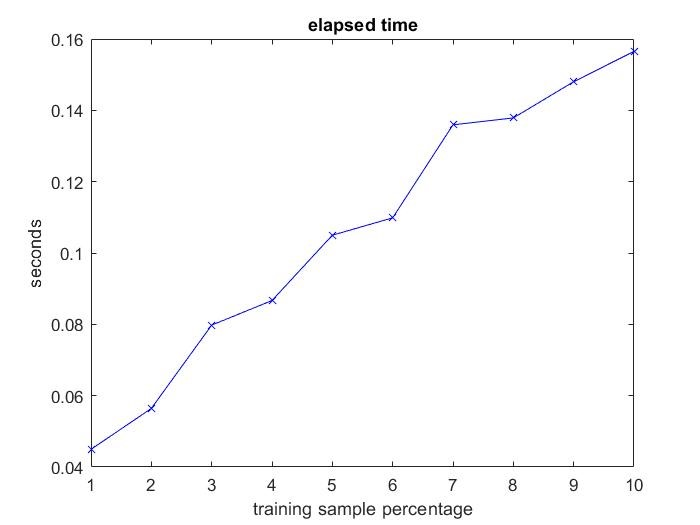
\includegraphics[width=0.6\textwidth]{figures/knncomp.jpg}
%	\caption{Computation Time}
%	\label{fig:knncomp}
%\end{figure}




%Figure~\ref{fig:knntest} shows that the test error decreases as the 
%training set becomes larger.









